\documentclass[12pt,a4paper]{article}

% Packages
\usepackage[margin=2.5cm]{geometry}  % Adjust margins as needed
\usepackage{url}
\usepackage{ragged2e}  % For left-aligning text
\usepackage{authblk}   % For multiple authors
\usepackage{hyperref}
\usepackage{longtable}
\usepackage{graphicx}
\usepackage{float}

\setlength{\parskip}{1em plus 0.2em minus 0.1em}
\setlength{\parindent}{0pt}

% Left-align all text
\RaggedRight



\begin{document}
% Title and author information
\title{HCI 1 Report Deliverable}
\author{Marcel Venturotti}
\author{Thomas Turner}
\author{Sam Wavish}
\affil{University of Bath}
\maketitle

\section{Introduction}

People over the age of 65 often face isolation due to physical limitations, distance from their loved ones or a lack of opportunities for social interactions. Many older adults have limited experience with technology so using our project may be challenging. The idea for this AR software aims to make it easier for older adults to socialise by offering them an easy-to-use platform that allows them to interact with friends and engage in social activities without having to leave their house. 
 
In England, 2 million people over the age of 75 go over a month without speaking to a friend, neighbour or family member (\cite{ELSA2024}). Isolating oneself can have detrimental effects on our mental health. Isolation and a decrease in socialisation are increasingly present for older people due to their elderly status rendering common socialising activities much more challenging. 

The main motivation behind this project is to reduce social isolation among older adults, being a way to improve their mental and physical wellbeing. By using augmented reality, we aim to make communication and socialising between their friends more accessible, improving their overall quality of life. 

Furthermore, after experiencing the social status of the world during COVID-19, when restrictions on in-person interactions highlighted the emotional and psychological impact of reduced social contact as well as the challenges of socialising online, we felt it appropriate to try and find a solution for this issue. 


The project is specifically designed for the 65+ age group, focusing on their challenges with mobility, use of technology and social interaction, using an AR system refined iteratively with a user centric design. Our design will be tailored to address common barriers older adults face, including lack of familiarity with technology, accessibility issues and so on.

Our stakeholders in many cases have limited experience with technology. They are also motivated by their desire for genuine interaction with others, but face challenges like difficulty travelling, which may be caused by physical health concerns or living far away from friends and loved ones. The software must fit easily into their daily lives, with a minimal setup and simplicity of navigation and usage. They may also have auditory, visual, and other impairments which should be considered in the design. 


The stakeholder's goal is to connect with friends and family in a way that feels natural and comfortable. They need an easy-to-use platform where they can easily engage in social activities with little to no prior technical knowledge. They need it to be simple and accessible, making sure that the software is not overwhelming for them. 


\section{Proposed Vision}

The problem domain guided us to design an innovative and interactive way to make socialising easier for older people based on needs elicited by stakeholders. The overall idea for the design is a glasses-based AR system with messaging (including calling) and game-playing features. The option to play music in the background is also provided to enhance and familiarise the experience with an in-person interaction. 

Physical hand gestures were preferred to select options in the virtual environment over alternative methods such as eye tracking or virtual controllers. \cite{Davis_2021} demonstrates that changes in the aging eye contribute to eye tracking difficulty in older persons, in particular macular degeneration, prevalent in 4.8\% of those aged 65 or older, and 12.2\% in those aged 80 or older, increasing the feasibility of physical gesturing as the primary mode of interaction. This was enabled using depth sensors, due to the limited computational power of current virtual glasses technology (i.e. Google Glass) \cite{Bikos_2015}, further discussed in our design section. 

A typical usage of our design would play out as follows. After mounting the virtual glasses, users are provided a contact list with all their friends they can call. Each friend’s profile will be represented by an icon or nameplate. They can select one or multiple friends to create a session with by virtually placing their finger over who they wanted to call. Ensuring sessions can be made as a group was very important for stakeholders, as a survey analysis confirmed they usually met multiple people at once when socialising in person. A confirmation step will be implemented for each selection to minimize errors, ensuring a stress-free setup process. 

In the group session, multiple options are offered to the user. They could choose to engage in a synchronous chat, with attendees rendered as their virtual avatar, but stakeholders expressed a strong preference for activities that simulate in-person interactions, in particular game-playing. Favourites of our target demographic included boardgames such as chess, and various card games. Therefore, we implemented the option to select 2+ player games that had a low barrier to entry in terms of skill and learning the system controls, but were still engaging (Chess, Blackjack and Scrabble). This was further informed by \cite{Chen_2020}, which elaborated on our choice for games, preferring those that are intellectually stimulating (i.e. puzzles), with much more precedence in the elderly population compared to violent or action-packed gameplay. The choice to include a game-playing element was also informed by this research as it relates to demonstrable improvement of cognitive performance and reducing rates of depression in the elderly using board games in augmented reality (\cite{CogARC2024}).

The user would be able to select a game in a similar fashion as the contacts. Before beginning to play, the rules of the game and how to play it in a virtual environment, would appear in everyone’s field of view. The users in the session can then play the game for as long as they wish. This is an extended design consideration based on the needs of our stakeholders, providing learning resources for each element of our application. This included a guided tour of the menu systems, as well as each individual game, which was both comprehensive and incorporated accessibility elements such as text-to-speech and icon magnification, to minimise the possibility of confusion or frustration using the system. This was informed by \cite{Thomas_2021}, which follows on from related research demonstrating that usability in AR systems is a key concern for involving the elderly population in this new technology. The study, aimed at individuals over the age of 50, showed that text and audio prompting, alongside ghost hand and ghost object prompting, was more effective than other types of visual prompting in interpreting virtual guides. This directed us to enable a transcribed audio guide and a visualisation of a hand (‘ghost’ hand) for physical gestures, for both game playing rules and menu systems. 

One example game we envisioned to be implemented in our system was Chess, which was selected due to its cultural and gender neutrality in comparison to many other puzzle games, alongside falling into the ‘intellectually stimulating’ category, which was deemed suitable for the elderly in the previous paragraph. As we selected physical gesturing as our initial primary mode of interaction, we based our design considerations on \cite{Bikos_2015}, utilising depth sensors to project a virtual chess board and emulate interactions between the user and virtual chess pieces. This required that both players involved selected a suitable table to ‘bind’ the board, allowing the system to then support real time synchronised moves and maintenance of game state. The ‘ghost hand’ technique was used to support the user in learning how to move the virtual chess pieces and ‘bind’ (position) the chess board on an appropriate surface. 

To render the overall experience more comfortable and familiar, we enabled the option for shared background music, as many of our stakeholders referenced using music for in-person game-playing interactions. Two options were provided: various classics from music genres prevalent in the 1950’s-2000’s, and the opportunity to connect with a personal Spotify account for those who were more tech-savvy. 

A very important element to incorporate based on the needs of our stakeholders was accessibility. Most presented disabilities such as hearing loss, mobility issues and partial blindness. \cite{Chris_2023} informed us in the design of accessibility features, in particular the development of speech bubble generation during and other visual communication methods. Approximately 80\% of individuals over the age of 70 present with hearing loss \cite{Michael_2024}, so this was a particular focus of ours. To further address these issues, we implemented text-to-speech and speech-to-text with a chat feature, as well as magnification of menu features such as selectable icons. This ensures features of our system are flexible and easy to use for the entire demographic, not just physically healthy elders.  

Finally, we needed to make some design considerations in terms of the presentation of digital avatars or likenesses of the users. \cite{Chris_2023} also informed our decisions here, by including survey data relating to how physical representations can lead to barriers to entry for AR/VR applications, as well as the ethics of freedom of choice in character selection. Further, \cite{Lin_2021} provided a study of exercise-based outcomes relating to the usage of youthful or elderly appearing avatars in augmented reality, which demonstrated that a focus on youthful appearances improved vitality and physical health outcomes in the elderly, which we believe will also contribute to improved efficacy of social interactions. Thus, we enabled customisation of various avatars across the full age spectrum, although highlighted more youthful characteristics, such as signs of fitness and expressivity in the avatars. 

We can justify the selection of augmented reality as our presentation method for a few reasons. Firstly, AR integrates virtual elements in the real world. Being able to call your friends and play your favourite games with them in a familiar environment greatly increases overall comfort and reduces disorientation. Further, AR minimizes the cognitive load required to navigate and interpret fully immersive environments, making it more user-friendly for this demographic \cite{Lee_2023}.

Secondly, using AR allows us to implement the ability to play games in an interactive and realistic way. Contrary to playing chess with a friend on a computer for example, the user can interact with virtual objects in the same physical space or through synchronized AR interactions. This creates a sense of presence and connectedness, which is critical for socialisation \cite{Laine_2022}. 

Finally, the use of AR allows the user to move around during the interaction which is beneficial for older adults by promoting physical activity and breaking monotony. Furthermore, always having your surroundings visible to you reduces the risk of physical hazards such as tripping or bumping into objects especially if some of our stakeholder presented mobility concerns \cite{Drakakis_2023}. 

\section{Requirements}

Requirements were obtained through combining responses from an unstructured interview with an individual from our target audience (70 years old, M), as well as a survey questionnaire. The unstructured interview focused on a few key questions, which framed the rest of the conversation. The entire conversation was transcribed in real time, and then some key insights and requirements were extracted using a thematic analysis. This involved ‘coding’ responses by extracting key phrases and repeated terms, then extracting latent content (subtext) from these codes, allowing us to identify the most important problems and benefits of our AR system for our target audience. The survey questionnaire included a range of open-ended, Likert scale items and multiple-choice questions, which was analysed both quantitatively and qualitatively. 
 

Requirements were prioritised based on the MoSCoW technique, which included the following categories: (Must Have; M) essential HCI requirements critical for usability and user experience, (Should Have; S) important HCI features that significantly enhance the interface but are not critical, (Could Have; C) desirable HCI elements that would improve the interface if time and resources allow, (Won't Have; not included; W) HCI features that are not necessary for the current version.

\begin{longtable}{|p{3cm}|p{3cm}|p{3cm}|p{3cm}|}
\hline
\multicolumn{4}{|c|}{Requirements} \\ \hline
Requirement ID & Description & Further Explanation & Priority \\ \hline
\endfirsthead % Header for the first page
\hline
Requirement ID & Description & Further Explanation & Priority \\ \hline
\endhead % Header for subsequent pages

\hline
R1 & Simplified and Intuitive User Interface (Buttons Only) & AFG & S \\ \hline
R2 & Accessibility Tooling & Audio localization, magnification for menu systems, speech bubble generation and other visual communication methods. & M \\ \hline
R3 & Physical and Virtual Guides & Physical handbook for necessary devices (i.e. Google Glass). Virtual guide including audio-text descriptions and demonstrations of a ‘ghost’ hand for game-playing and menu interaction. & M\\ \hline
R4 & Supports Group Interaction & Providing synchronous group communication support, such as shared game-playing sessions. & M\\ \hline
R5 & Background Music & Providing custom song selection or shared song selection for group sessions during gameplay. & C \\ \hline
R6 & Gameified Interaction (Active Involvement) & Our system should be focused on enabling social interaction through games such as Chess and Scrabble. & M \\ \hline
R7 & Familiarity and Seamless Merging with Real Environment & ... & S \\ \hline
R8 & Accommodation of Game Selection and Music Selection based on Varied Cultural Backgrounds  & Games to be representatively sampled to include culturally specific examples (). Likewise for music.  & S \\ \hline
R9 & Minimal Cognitive Load & This is related to simplicity in the user interface. For example, menu layout should be minimal, fonts should be uniform, general UI elements should be similar across the entire application & S \\ \hline
R10 & Physical Interaction Support (Gesture Recognition) & Game-playing and menu selection is supported mostly by gesture-based interactions (i.e. moving hand forward, finger tapping a virtual ‘holographic’ screen.  & M \\ \hline
\end{longtable}


\section{Design, Implementation and Feedback}

To reach our high-fidelity prototype from which we produced our video prototype, we completed two prototype and feedback cycles. These allowed us to propose prototypes and obtain feedback from stakeholders in a user-centric manner.  

After brainstorming our ideas for our design, we formed a survey questionnaire and unstructured interview to obtain needs from our stakeholders. For the survey, we ensured it maintained full user anonymity; Microsoft Forms automatically hides respondents email addresses. Microsoft Forms also supports views and data analysis obtained in a clear and efficient manner, such as pie charts showing the spread of the responses and averages for numbered responses showing clearly the key information, avoiding the need for us to transfer responses and process manually in tabular data software such as Excel. 

The survey was composed of three sections: socialising, technology and requirements. Only the first section was obligatory to fill, allowing the survey to be short, in case the stakeholder does not have time to fill in all the sections. We used a variety of methods to obtain responses: Likert scales, text boxes for open-ended responses and multiple-choice items. This provided us with very useful insight into what the elderly do when they socialise, how familiar they are with technology and what they would need from our design.  

One multiple-choice item prompted the potential user’s proficiency level with technology in one of four categories, with some provided examples of expected ability for each category (Beginner, Intermediate, Advanced, Expert). Most respondents claimed Beginner status (~83\%), a small proportion claimed intermediate status (~17\%), and no respondents claimed Advanced or Expert status. This further demonstrated the need for physical and virtual guides to support learning how to use our system, which informed the development of assistive learning features (including a voice over and descriptive pop-ups). 

Problematically, response rates and feedback amount were limited, a major limitation of questionnaires. This is why we also conducted an unstructured interview, allowing us to collect more detailed responses and extract more specific requirements. One example of a benefit the concomitant interview provided was the elicitation of accessibility needs, which was incorporated extensively in our design.  

In a section of the interview transcript, the interviewee was guided to discuss difficulties they face in real life socialization that could be improved with the use of this type of technology. Themes noted were references to physical disabilities, such as hearing and visual impediments, for example ‘sometimes I have a difficult time comprehending what my friend is saying to me when we go to the pub on a busy day of the weekend’, and 3-4 repeated concepts (i.e. low volume, difficulty zooming). This makes accessibility tooling especially important as a requirement, in particular localizing and enhancing audio, large default font and icon sizes with the option to magnify, and so on – which were confirmed as useful accessibility support mechanisms with the interviewee in real time. 

This marked the initial design stage of our first iteration of UCD. Then, using the requirements and data collected, we came up with our low-fidelity prototype. Despite some initial positive feedback and signs of interest from our stakeholders, they did not fully comprehend how our design would be used, due to their general lack of familiarity with AR systems. Therefore, we designed a storyboard to demonstrate usage, enabling us to support and iteratively redesign our product with newly elicited requirements and suggestions. 
 
The comic described, in 6 sketch boxes, the typical use case of our design. This began with a depiction of an older adult who is lonely and temporarily separated from normal social activities that sustain them, flowing through to a demonstration of how their needs could be met even in distanced interaction because of using our system. Once created, we performed a cognitive walkthrough of our storyboard with stakeholders, explaining to them frame by frame how our system operates. The cognitive walkthrough is a technique for evaluating our systems capacity to be taught from the perspective of a brand-new user, allowing us to focus on the thought process of the user as they interact with our system, helping us identify usability issues early \cite{Concept2023}. 

We asked them if they felt it aligned with their needs, if the flow made sense, if features were clear. Stakeholders expressed high clarity when it came to the usability of our design, but raised interest in how accessible our design would be. This was a valid point as we were unable to delve deep into the technical features in our low fidelity prototype. This evaluation concluded the first iteration of prototyping and feedback.  

From there, we felt our high-fidelity prototype had to emphasize user accessibility, demonstrating features which were elicited from our interview analysis. Indeed, after presenting our low fidelity prototype users raised concern about how our design handled various impairments, with some stakeholders presenting with hearing loss, mobility impairments and visual impairments. 

Utilising this feedback, we progressed to designing our high-fidelity model, covering the prototype in more detail and reducing confusion in terms of usability and technical details, such as accessibility supports. Obtaining this secondary feedback (following initial requirements elicitation) was crucial in constructing a new design that focused on the most important aspects of the system, based now on stakeholders deeper understanding of the potential final product. This emphasises our focus on a user-centric design. 

Through multiple design iterations we tried to accommodate as many accessibility requirements as we could, but limited support could be provided in some instances. For example, a large component of our product was gamified interaction, which relies heavily on physical gesture-based interactions. Some of our stakeholders presented with mobility issues and eye tracking issues concurrently, and for this group, we could not provide an effective modality for playing many supported games. 

We determined the best way to demonstrate our product and get evaluative feedback would be to propose a meeting with our stakeholders directly, utilising the Wizard of Oz technique, built to simulate how users interact and respond to final product features. The Wizard of Oz technique is a widely used research method in Human-Computer Interaction where participants interact with a system that appears to be autonomous, but in fact, the system is being operated or controlled by a human behind the scenes (the "wizard").  \cite{Paul1985}.

We utilised Figma (a low-code website frontend design tool) to create a virtual UI as a demonstration of our high-fidelity prototype. Multiple designed menus and views were displayed to the user, including contact, music and game selection, accessibility options as well as confirmations pop-ups. This was while someone else shared the page with real-time modification access, which enabled fine-tuning of UI elements, and simulating interactions such as button presses and state transitions (in implementing the WoZ technique). For example, when the font magnification accessibility button was interacted with, we could simulate the effects of this button press and any following state transitions (moving out of the accessibility menu to the home menu). With this process we were able to directly talk to the user as they interacted with the webpage, obtaining immediate impressions and concerns. 

Our goal was to ensure the application’s accessibility to the widest possible range within our demographic. While it can't be accessible to everyone, we prioritised features that would have the greatest impact, even if that meant trading off other potential functionalities. To do this, we constructed a final follow-up survey for those presenting with various disabilities that flagged possibly usability issues during our WoZ study, including Parkinson’s disease (and other motor impairments), auditory impairments and visual impairments. As mentioned previously, many of the recommended supports raised included implementing resizing for icons and fonts, visual guides and prompts alongside voiceover prompts, and minimising the clutter of the menu layout. In the end, this also supported the minority, as a few stakeholders presenting with Parkinson's disease expressed improvement of usability when navigating with larger icons and diffuse menu layouts. 

The high-fidelity prototype directly reflects on what the stakeholders need since it was built on the feedback collected from them during the low fidelity prototyping stage. Through their feedback we were able to include features that directly address the key concerns raised by the stakeholders, such as making it a clear and easy to use interface. For the prototypes we focused on designing and demonstrating the features that the demographic would need knowing their challenges such as limited technology experience or physical impairments. 

 That is why we found it crucial to include features such as adjustable font sizes and a simplified navigation to make the experience as easy as possible for the stakeholders. With our high fidelity prototypes we were able to allow the users to interact with the core functionalities in a simplified way and able to use their feedback on parts they struggled with and parts that they appreciated in helping them use the prototype. The prototype gave great feedback as it mimics the real-world scenario of them using the application allowing them to relate to the product easily, ensuring the prototype isn't just theoretical but practical and applicable to them.  

\begin{figure}[H]  % The 'H' argument suggests placing the figure here
  \centering
  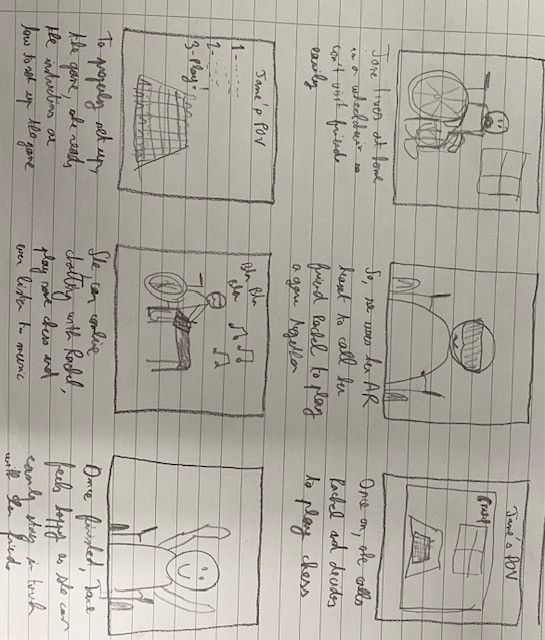
\includegraphics[width=0.7\textwidth]{story.jpg}  
  \caption{User story board}
  \label{fig:story_board}  
\end{figure}


\begin{figure}[H]  
  \centering
  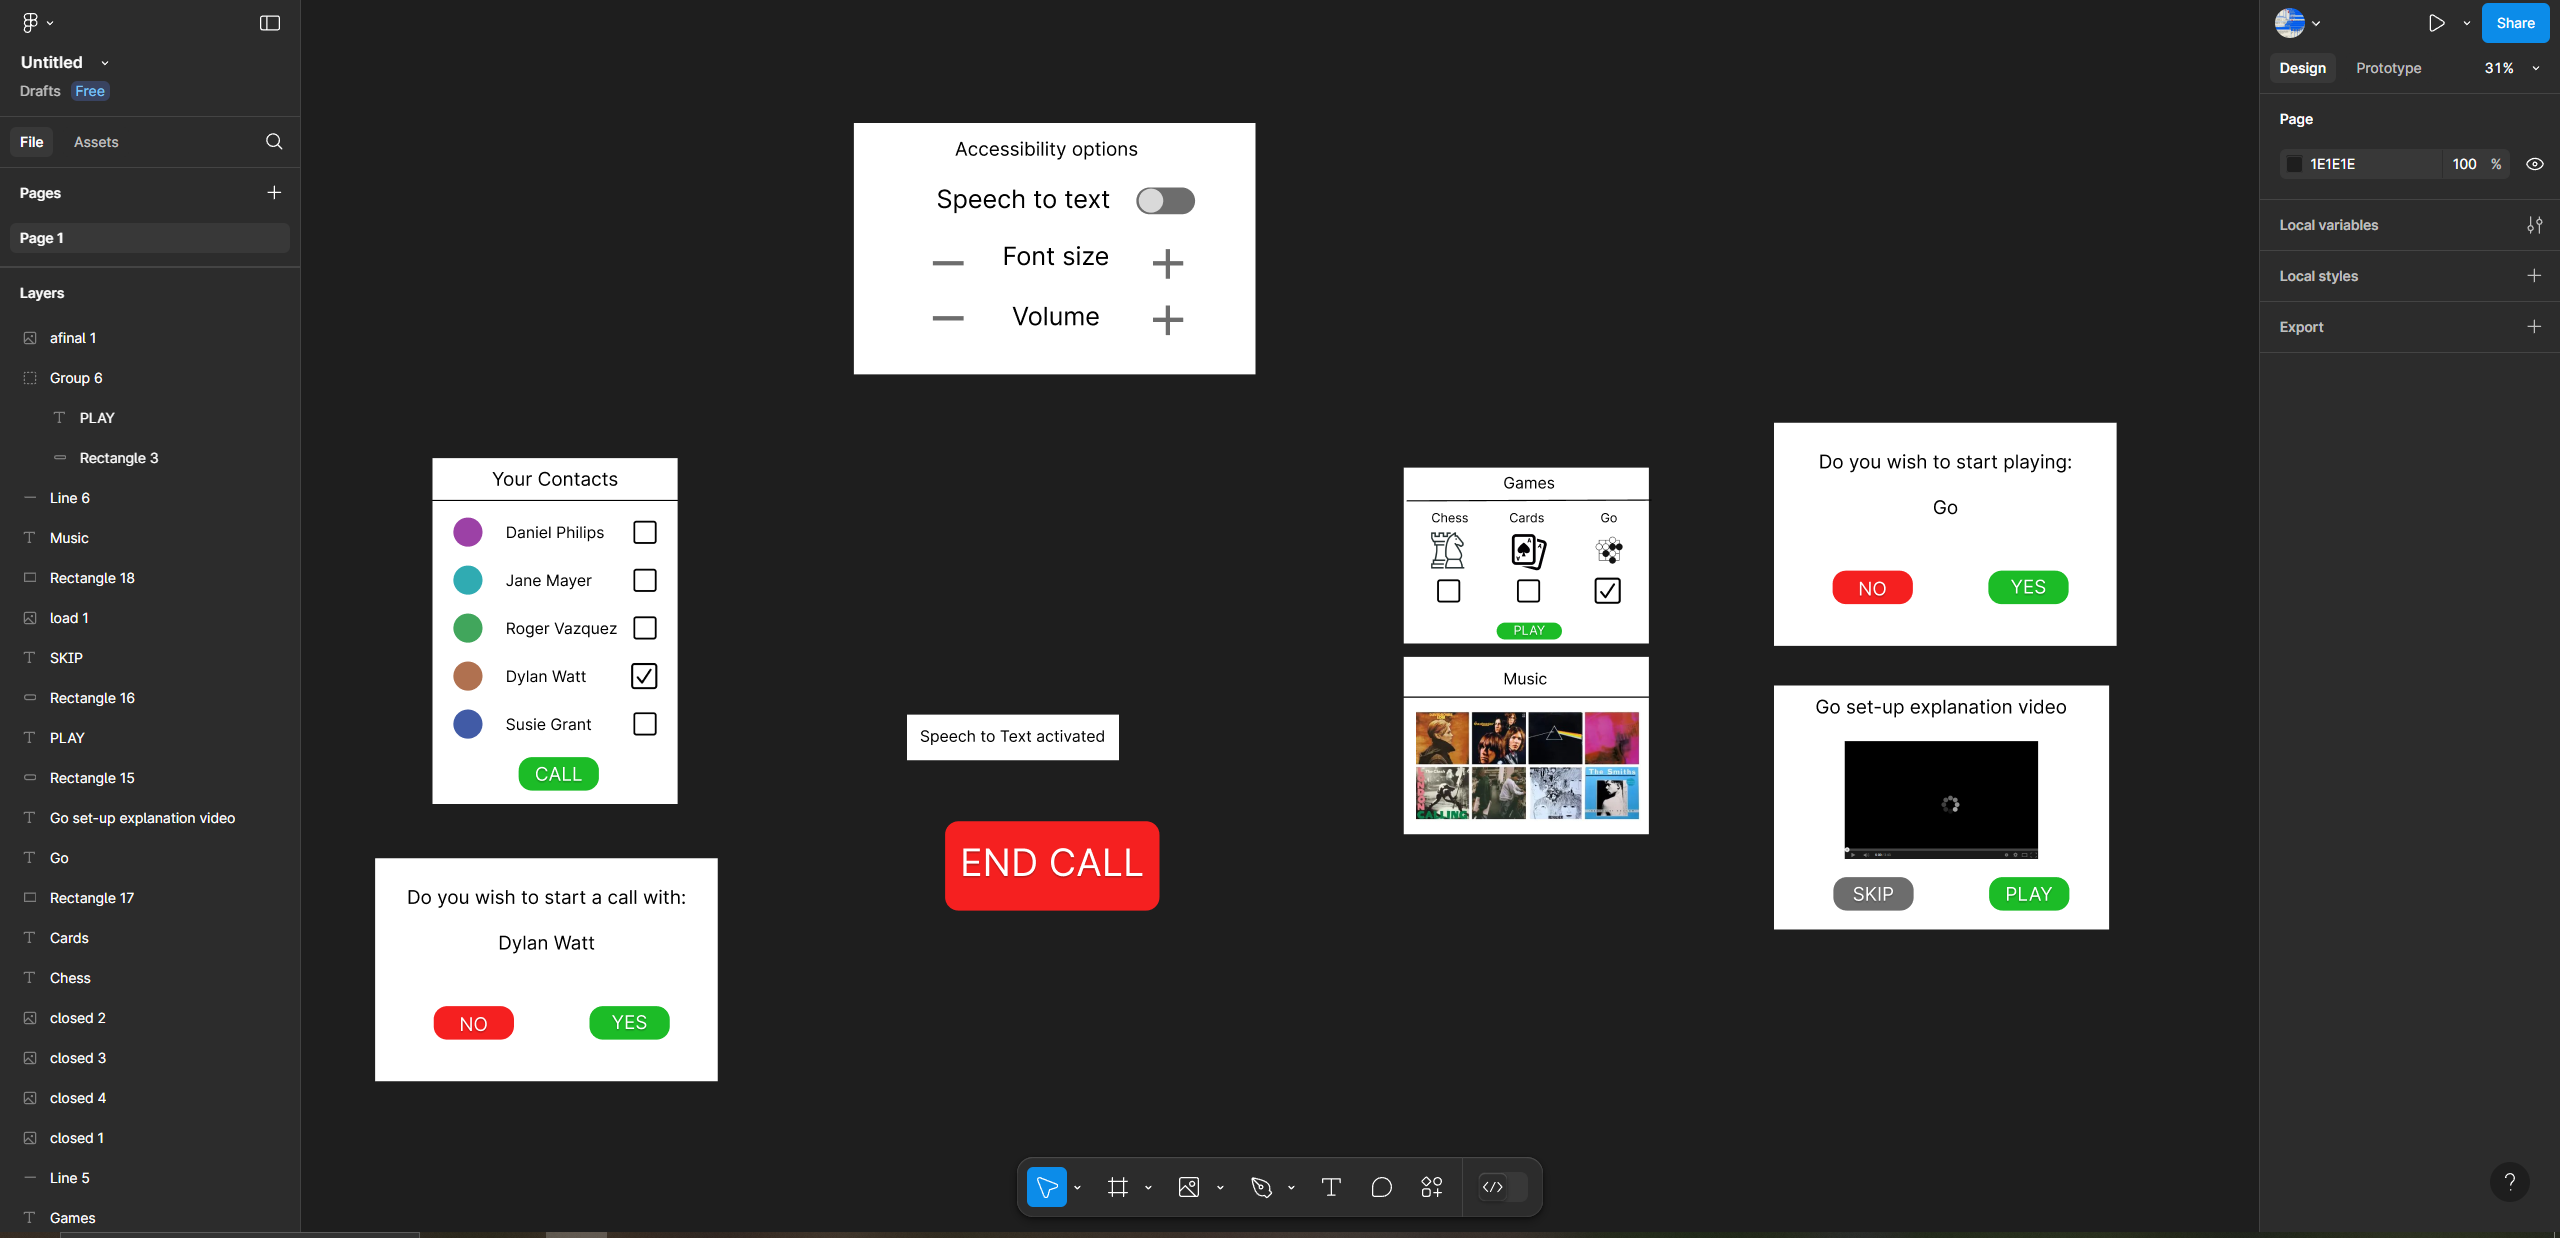
\includegraphics[width=0.7\textwidth]{HFP.png}  
  \caption{High fidelity prototype with Figma}
  \label{fig:high_fidel_proto}  
\end{figure}

\begin{figure}[H]  
  \centering
  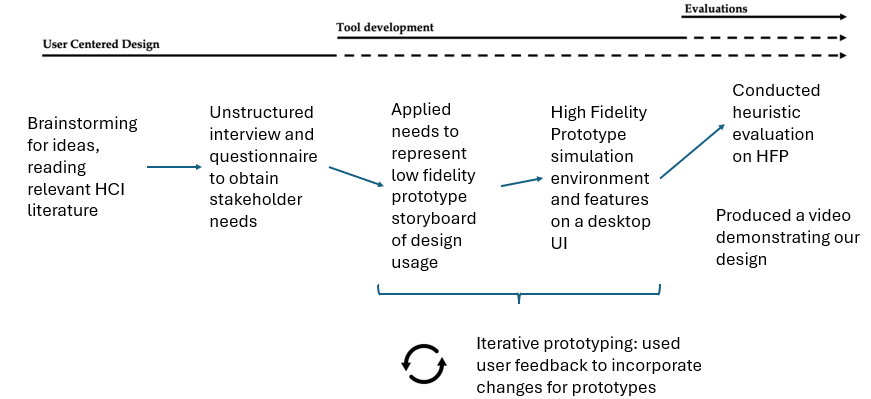
\includegraphics[width=0.7\textwidth]{workflow.png}  
  \caption{UCD Workflow}
  \label{fig:workflow}  
\end{figure}

\begin{figure}[H]  
  \centering
  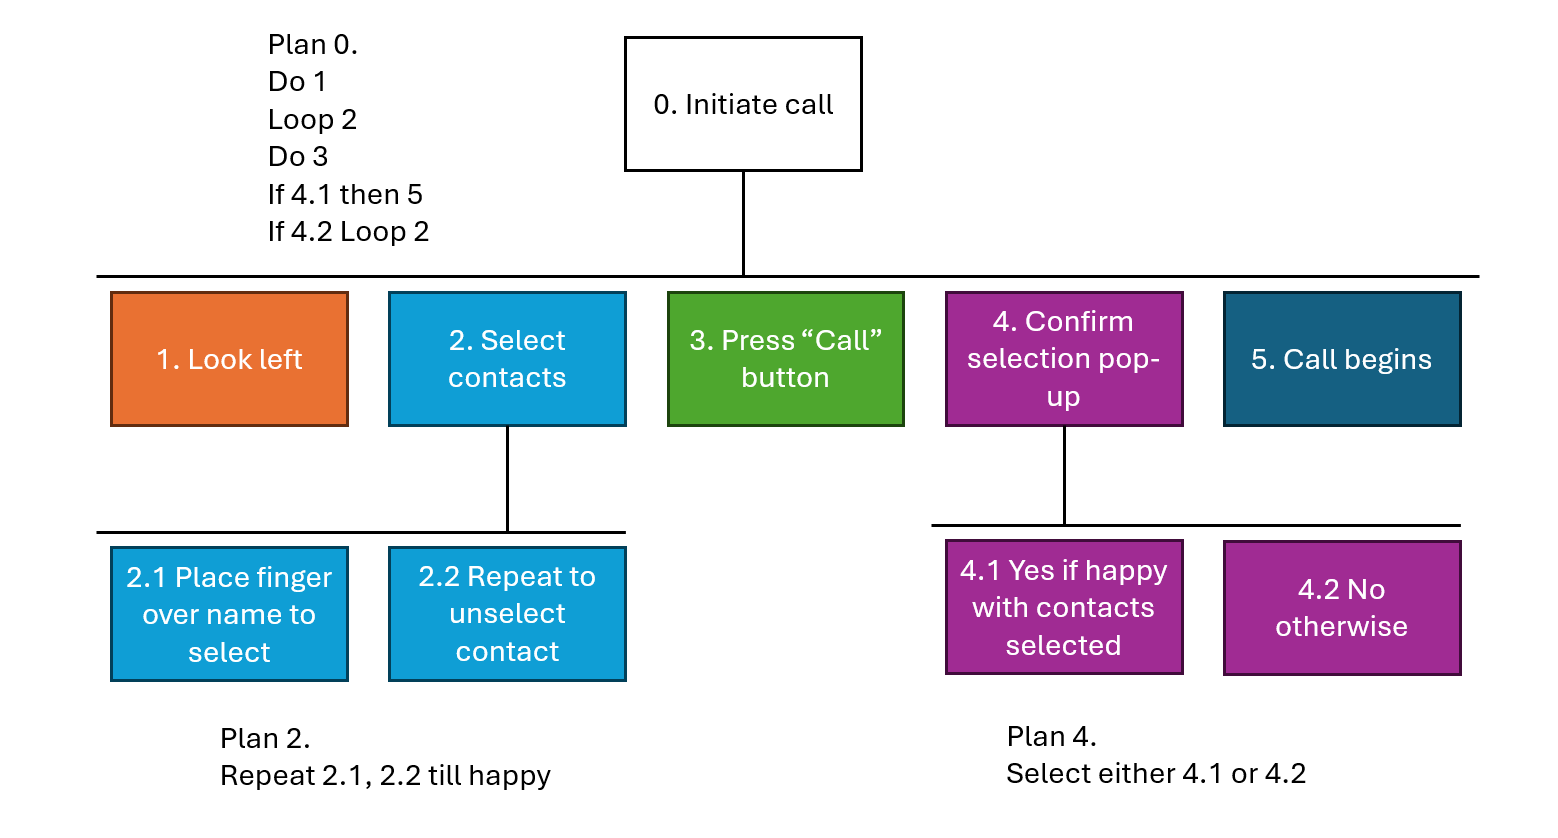
\includegraphics[width=0.7\textwidth]{hta.png}  
  \caption{Hierarchical Task Analysis}
  \label{fig:hta}  
\end{figure}


\section{Evaluation}

We conducted one formal evaluation on our first high fidelity prototype, which allowed users to interact with the interface on a desktop UI, emulating but not directly demonstrating the AR element. This permitted them to get a feel for the positioning and functionality of features in the AR environment, without being initially overwhelmed by complexity. We chose a heuristic evaluation as it is an effective way to obtain feedback and improvements on various defined aspects of our high-fidelity prototype. Also, as this prototype was designed on a desktop, a heuristic evaluation is known to be primarily designed for this case.  

We applied Schneiderman’s eight golden rules (obtained from his book publication "Designing the User Interface: Strategies for Effective Human-Computer Interaction", 1987), as it primarily focuses on interaction design. The heuristics allow stakeholders to clearly identify problems and their severity for the major aspects of our high-fidelity prototype. The eight heuristics defined for our formal evaluation were: strive for consistency, seek universal usability, offer informative feedback, design dialogs to yield closure, prevent errors, permit easy reversal of actions, keep users in control and finally reducing short-term memory load.  

Stakeholders were able to identify a couple of issues with our prototype which really helped us layout our video prototype simulating the real AR experience. All their observations were stored in a spreadsheet where we noted the problems, their severity and what we could do to improve it for each heuristic.  

We learnt that when they were asked as to whether they find the design predictable and easy to navigate, they mentioned that despite the simple and clear interface, some fonts weren't uniform which led to excess cognitive load. However, we received mostly positive feedback about the accessibility due to incorporating settings for a variety of common impairments.  

Finally, even though we had set up the option to undo choices in case of errors, they recommended the incorporation of confirmation messages, such as mentioning the call has ended, or that the game has been correctly selected. They marked this as more important than previous observations and problems as this change would really allow to make the usage much clearer and emphasize closure of actions.  

This formal evaluation allowed us to incorporate these recommendations into our video. We had to ensure that fonts maintained a regular scalable size. We also add confirmations messages for the contact selection, accessibility changes, game selection and the end of a call. This took the form of either boxes confirming their choice allowing the possibility to go back in case an error (“Do you wish to call XYZ”, followed by red and green yes or no options), or simple text pop-up presenting the change they have made (such as: “Font size increased” or “Call ended”).  

\section{Discussion and Conclusions}

To conclude, we were able to implement a high-fidelity prototype and an explanatory video of our proposed vision through two iterations of the design-prototype cycle. During every stage of the process, we always went back to stakeholders to obtain valuable feedback to move on efficiently and respect the user centred design paradigm. 

One issue is that in the design process, we were limited by time. We spent much time obtaining initial needs from stakeholder as well as feedback from our high-fidelity prototype. In particular, enabling a large sample to participate in the WoZ method was very time and resource consuming.  

For future work on this design, we would have used the feedback form our formal evaluation to design a second high-fidelity prototype. In the two iterations we performed, the majority of our focus was aimed on the interface design, ensuring its accessibility to all stakeholders. Therefore, if we were to implement a second high-fidelity prototype, a change of direction would have been made centred around the game functionality, explaining its functionality in more depth, and how users can interact with it.  

Finally, the design process for this AR application differs quite drastically from a traditional mobile or web application. To begin with, having to prototype with a medium very unfamiliar to stakeholders involves having to spend more time and resources explaining the capabilities of and generally how to use the system. This step can be completely overlooked when working on a mobile or web application as most stakeholders are already familiar with that environment. 
	
Furthermore, when implementing prototypes for AR designs, designing it in the AR environment comes much later in the process. We had to first create our high-fidelity prototype on a desktop for stakeholders to engage in it to offset the initial learning curve to familiarise with the system, including gesturing. This creates the need for extra iterations of the design process rendering AR/VR applications much more complex to design over traditional mobile or web applications.  


\bibliographystyle{ACM-Reference-Format}
\bibliography{references}

\end{document}
